%!TeX TXS-program:bibliography = txs:///biber
\documentclass[10pt,letterpaper]{article}
\usepackage[latin1]{inputenc}
\usepackage{graphicx}
\usepackage{listings}
\usepackage{hyperref}
\hypersetup{
	colorlinks,
	linkcolor={black},
	citecolor={black},
	urlcolor={blue}
}
\usepackage{float}
\usepackage{acronym}

\acrodef{DOI}{Digital Object Identifier}
\acrodef{DC}{Dublin Core}
\acrodef{PSID}{Panel Study of Income Dynamics}
\acrodef{ICPSR}{Inter-university Consortium for Political and Social Research}
\acrodef{CMS}{Content Management System}
\acrodef{HCI}{Human-Computer Interaction }
\acrodef{DAS}{Data Accessibility Statement}
\acrodef{FAIR}{Findable, Accessible, Interoperable and Reusable}
\acrodef{FSRDC}{Federal Statistical Research Data Center}
\acrodef{FTI}{Federal Tax Information}
\acrodef{NSO}{National Statistical Organization}
\acrodef{LBD}{Longitudinal Business Database}
\acrodef{PID}{persistent identifier}
\acrodef{AEA}{American Economic Association}
\acrodef{API}{Application Programming Interface}
\acrodef{CSS}{Cascading Style Sheets}
\acrodef{URL}{uniform resource locator}
\acrodef{IDCC}{International Digital Curation Conference}
\acrodef{RDA}{Research Data Alliance}
%\usepackage{natbib}
\usepackage[sorting=nyt,maxnames=10,backend=biber]{biblatex}
\addbibresource{references.bib}

\author{Lars Vilhuber and Carl Lagoze}
\title{Supplementary Materials}
\begin{document}
	
\section{Scenario 1}
We know the \ac{DOI} of the article, it's hosted at openICPSR: \url{http://doi.org/10.3886/E100590V1}
\lstset{numbers=left,numberstyle=\tiny,stepnumber=2}
\begin{quote}
	\it
McKinney, Kevin L., Green, Andrew S., Vilhuber, Lars, Abowd, John M., and Abowd, John M. Replication data: Total Error and Variability Measures for QWI and LODES. Ann Arbor, MI: Inter-university Consortium for Political and Social Research [distributor], 2017-12-15. https://doi.org/10.3886/E100590V1
\end{quote}

We note that this dataset, as all current openICPSR datasets, is licensed under a \href{http://creativecommons.org/licenses/by/4.0/}{Creative Commons Attribution 4.0 International License}. 

\subsection{DataCite}
\lstinputlisting[language=xml,linerange=1-9]{datacite-api-100590.xml}
\lstinputlisting[language=xml,linerange=10-10,firstnumber=10,basicstyle=\bfseries]{datacite-api-100590.xml}
\lstinputlisting[language=xml,linerange=11-22,firstnumber=11]{datacite-api-100590.xml}
\lstinputlisting[language=xml,linerange=23-24,firstnumber=23,basicstyle=\bfseries]{datacite-api-100590.xml}

Reveals the identity of the \texttt{datacentre} or the \texttt{publisher}. There is no information on the license under which the object is made available, no copyright holder, or any information on persistence of the data.

\subsection{re3data}
If one were to successfully lookup ICPSR on re3data \parencite{re3data}, we would find  \url{https://www.re3data.org/repository/r3d100010255} \parencite{Re3data-icpsr}.
\footnote{To be more precise: a lookup for the contents of the \texttt{datacentre} field yields 0 results. A search for the contents of the \texttt{publisher} field yields a wrong result (\lstinline|<odesi>|). We applied human judgment. } Three types of data access are listed. Furthermore, three data licenses are listed: two \texttt{other} and one \texttt{copyright}.
\begin{figure}[H]
	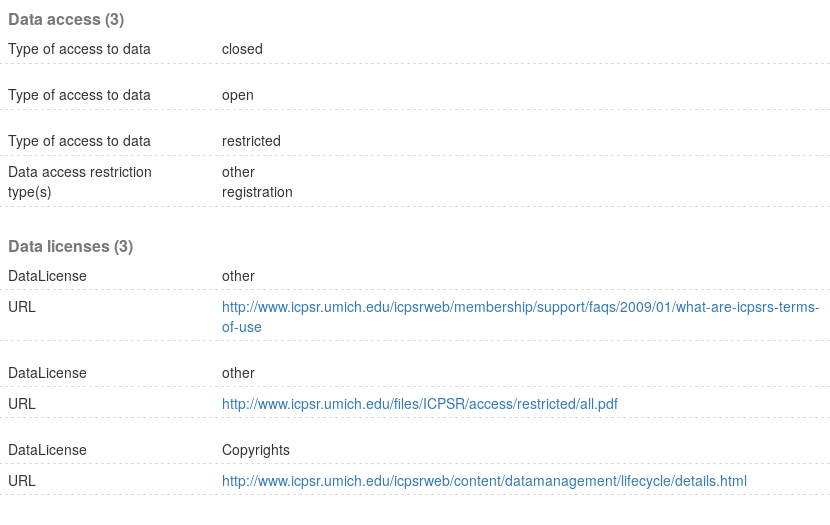
\includegraphics[width=1\textwidth]{re3data-org-icpsr-access-licenses-20181008.png}
	%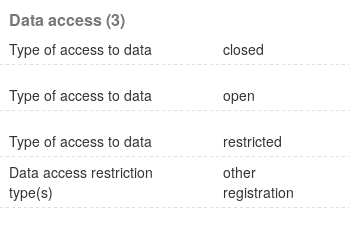
\includegraphics[width=0.4\textwidth]{re3data-org-icpsr-access-20181008.png}
\end{figure}

We would thus need to query the user about which license, and which access policy, applies to the particular dataset at hand. Note further that re3data makes no mention at all of the CC-BY license, which should, at a minimum, be an option.

\subsection{Data publisher website}
If instead we ignore the metadata on DataCite and re3data, and we go directly to the landing page indicated by the \ac{DOI}. The page offers four types of metadata: the in-page metadata, a link to a OAI-PMH record, a link to a DDI 2.5 record, and a link to a DDI 3.1 record.

The webpage itself lacks \ac{DC} metadata fields, but it does have identifiable fields for a license, using the \texttt{rel} identifier within the \lstinline|a| link field:
\lstinputlisting[language=xml,]{extract-webpage-20181008.xml}

However, no further information about persistence is provided on the page. The openICPSR FAQ contain such information, but do so somewhat obliquely, and do not point to a policy. Browsing the website, one might encounter the ``\href{https://www.icpsr.umich.edu/icpsrweb/content/datamanagement/preservation/policies/index.html}{Digital Preservation Policies and Planning at ICPSR}'' \parencite{icpsr-preservation}, which is not listed on re3data, and lays out the policies. 

\section{Scenario 2}
Restricted access at the \ac{PSID}. 
\begin{itemize}
	\item Access procedures at \url{https://simba.isr.umich.edu/restricted/ProcessReq.aspx}  - not mentioned anywhere on re3data
	\item re3data page at \url{https://www.re3data.org/repository/r3d100011131}
\end{itemize}
Note that none of these are versioned, and so do not describe how authors might have accessed the data 5 years ago (e.g., on a disconnected computer in their office - no longer an option, but also not documented as having been an option in the past).

\section{Scenario 3}
Restricted access at the U.S. Census Bureau.

%\bibliographystyle{chicagoa}
%\bibliography{references.bib}

\end{document}
